\pagelayout{margin}
\setchapterstyle{kao}
\setchapterimage{chargers-title3}
\setchapterpreamble[u]{\margintoc}
\chapter{Data}
\label{ch:data}

\footnotetext{Title image is a map of Prague with all chargers denoted as triangles in available datasets. The layer below displays all buildings in Prague with color being the number of floors}

This chapter introduces the data sources and processing methods that form the foundation of our research on electric vehicle charging demand. We begin by classifying the types of data used in our analysis and explaining their relevance to the research problem. We then describe the charging infrastructure data, including chargers and charging sessions, and detail how we transform this raw data into the target variables for our predictive model. Finally, we present the spatial and contextual data sources that provide the features for our model, along with the transformations applied to prepare them for analysis.

The data landscape presented here directly supports the modeling approach described in Chapter \ref{ch:problem}, where these processed datasets serve as inputs to our neural network with latent profiles.

\begin{kaobox}[frametitle=Types of data]

    \begin{itemize}
        \item \textbf{Spatial} (geospatial) data are those which have assigned position in real world and are invariant in some timeframe. Such data are locations of \acrlong{CS}, administrative boundaries, road network, buildings.
        \item \textbf{Temporal} data are characterized by their variation over time without specific geographical coordinates. In this thesis, these include charging session durations, energy consumption patterns throughout the day, historical charger utilization rates, and seasonal variations in charging demand.
        \item \textbf{Spatio-temporal} data incorporate both location and time elements, providing insights into how phenomena evolve across space and time. Examples relevant to this research include mobility patterns of people, real-time charger availability, and dynamic variations in \acrshort{APC} across different city zones during different hours of the day.
    \end{itemize}
\end{kaobox}

\section{EV Chargers and Charging Sessions}

\subsection{Description}

\begin{figure}
    \includegraphics[width=1\textwidth]{data/charger-ontology.png}
    \caption{A charging ontology showing the relationships between entities in the EV charging ecosystem}
    \label{fig:charging-ontology}
\end{figure}


To introduce our problem domain and establish a framework for connecting the various data elements, we present a simple charger ontology \sidenote{Ontology describes subjects of some system and the ways they are related to each other.}. Inspired by the AURORAL EV-charger Ontology \sidecite{OntologyDocumentationGenerated}, this ontology helps clarify the relationships between entities in the EV charging ecosystem. The model aligns with the data obtained from PRE (Prague's electricity distribution company).

Below is a description of the individual components of the charging ontology as illustrated in Figure \ref{fig:charging-ontology}.

\begin{itemize}
    \setlength\itemsep{1em}
    \item \textbf{\acrlong{CS}} (as visible in Figure \ref{fig:charging_station}) is equipment that connects an \acrshort{EV} to a source of electricity to recharge them. A charging station typically consists of physical infrastructure including power conversion hardware, connectivity modules, authentication systems, and user interfaces. Charging stations vary in their power delivery capabilities, ranging from slow AC chargers (3.7-22 kW) commonly found in residential and workplace settings to fast DC chargers (50-350+ kW) deployed in public corridors and commercial hubs. Within our dataset, charging stations from PRE's network predominantly consist of public AC and DC installations distributed throughout Prague's urban and suburban areas.

          \begin{marginfigure}
              \centering
              \includegraphics[width=0.42\textwidth]{data/charger-small.png}
              \caption{Picture of \acrlong{CS}. It has one connector on each of its sides. One of which has charging cable attached.}
              \label{fig:charging_station}
          \end{marginfigure}
          \vspace{3.5mm}
          Formally, we define the set of all charging stations as $S = \{s_1, s_2, ..., s_m\}$, where each station $s \in S$ is associated with a location $l_s \in \mathbb{R}^2$ representing its geographic coordinates.

    \item  \textbf{\acrlong{CP}} (as visible in Figure \ref{fig:charging-connector}) one or many are part of a \acrshort{CS}. These physical interfaces allow for the actual connection between the vehicle and the charging infrastructure. Connectors follow different standards depending on region and charging speeds. Each connector type supports specific charging protocols and power levels. In our studied network, the majority of charging stations feature multiple connectors, enabling simultaneous charging of different vehicles and supporting various connector standards to accommodate the heterogeneous EV market.

          \begin{marginfigure}
              \centering
              \includegraphics[width=0.3\textwidth]{data/charger-conector-small.png}
              \caption{View of 1 of the 2 charging connectors the \acrshort{CS} has}
              \label{fig:charging-connector}
          \end{marginfigure}
          \vspace{3.5mm}
          For each station $s \in S$, we define the set of connectors as $C_s = \{c_1^s, c_2^s, ..., c_{n_s}^s\}$, where $n_s$ represents the number of connectors at station $s$. Each connector $c \in C_s$ has a unique identifier $\text{id}^{c,s}$ assigned by PRE.

    \item \textbf{\acrlong{CSS}} occurs when an \acrshort{EV} arrives at a \acrshort{CS} and connects to a \acrshort{CP}. This interaction initiates a session that is logged by the \acrshort{CS} together with various parameters including connection time, disconnection time and total power consumed. The charging session captures both spatial, temporal patterns (duration, time of day, day of week) and energy consumption behaviors.

          \vspace{3.5mm}

          For each connector $c \in C_s$ at station $s$, we define the set of charging sessions as $V_{c,s} = \{v_1^{c,s}, v_2^{c,s}, ..., v_{k_{c,s}}^{c,s}\}$, where each session $v_i^{c,s} = (t_{\text{start},i}^{c,s}, t_{\text{end},i}^{c,s}, p_i^{c,s})$ is characterized by its start time, end time, and energy consumed during the session.

    \item \textbf{Location} denotes the geographical position where the charger is installed. This spatial attribute is crucial to our analysis framework as it allows for correlation between charging demand and various features of the surrounding environment.

          \vspace{3.5mm}

          The location function $l: S \rightarrow \mathbb{R}^2$ maps each station $s \in S$ to its geographic coordinates.

\end{itemize}

\subsubsection{Power consumption assumption}

\begin{marginfigure}
    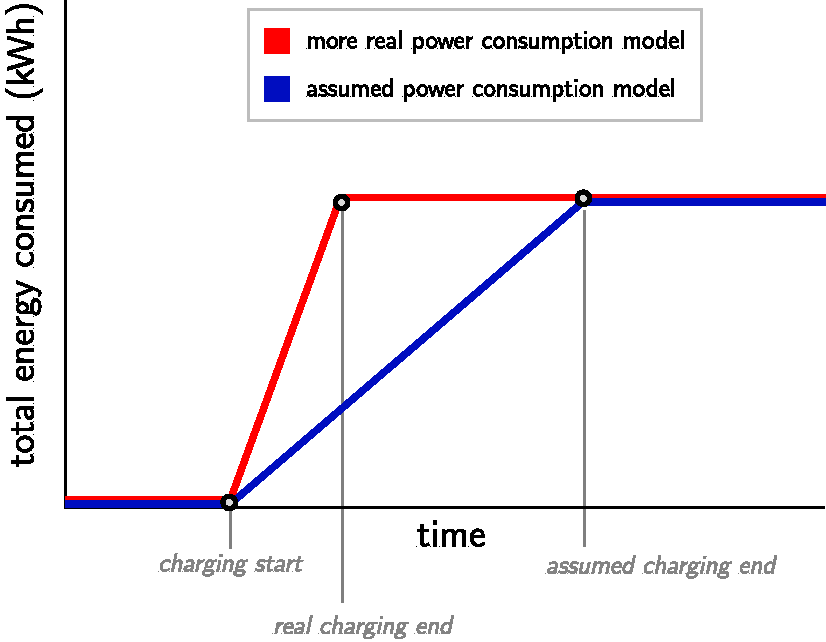
\includegraphics{charging-assumption.pdf}
    \caption[Charging assumption]{Chart comparing realistic power consumption vs our assumption.}
    \label{fig:charging-assumption}
\end{marginfigure}

Before we describe how \acrlong{CSS} have been processed into \acrlong{HPC} and \acrlong{APC}, it's important to clarify our simplifying assumption regarding power consumption during charging sessions. In reality, power consumption can vary significantly during a charging session, typically following a non-linear pattern. However, for modeling purposes, we make the following assumption:

The vehicle, from connection time, is charged at the maximum power that both the \acrlong{EV} can handle and the \acrlong{CP} can provide. This leads to charging sessions being divided into two distinct phases:
1. A charging phase, during which power is actively delivered to the vehicle
2. An idle period, where the vehicle has been fully charged but remains connected, consuming no power\sidenote{Some charging station providers financially penalize this idle period, as another \acrshort{EV} could be charging during this time. This practice can lead to improved availability of \acrlong{CS}.}

This simplification is illustrated in Figure \ref{fig:charging-assumption}, which contrasts our rectangular approximation with a more realistic charging curve.

\subsection{Charging Sessions Dataset}

PRE provided us with charging session data collected from \textbf{907} charging stations across Prague. We collected \textbf{385,404} individual charging sessions spanning  \textbf{January 2022 - June 2024}. For each session, the following information is available:

\begin{itemize}
    \item \textbf{Charger ID}: A unique identifier assigned by PRE to each charger and connector
    \item \textbf{\acrlong{CS} location}: The physical address of the charging station
    \item \textbf{Connector type}: Categorized as AC, DC, or UFC
    \item \textbf{Session timestamps}: Start and end times of each charging session
    \item \textbf{Energy consumption}: Total power consumed during the session
\end{itemize}


We identified the precise location of chargers using supporting documentation from PRE.

\begin{figure}[]
    \includegraphics{data/all-chargers.png}
    \caption{Map of all PRE \acrlong{CS} in Prague for which we have available \acrlong{CSS}. See Figure \ref{fig-large:all-chargers} for larger image.}
\end{figure}

\begin{marginfigure}
    \begin{tabular}{cc}
        \includegraphics[width=0.45\marginparwidth]{data/timelapse/timelapse0000.png} &
        \includegraphics[width=0.45\marginparwidth]{data/timelapse/timelapse0001.png}   \\
        \includegraphics[width=0.45\marginparwidth]{data/timelapse/timelapse0002.png} &
        \includegraphics[width=0.45\marginparwidth]{data/timelapse/timelapse0003.png}   \\
        \includegraphics[width=0.45\marginparwidth]{data/timelapse/timelapse0004.png} &
        \includegraphics[width=0.45\marginparwidth]{data/timelapse/timelapse0005.png}   \\
        \includegraphics[width=0.45\marginparwidth]{data/timelapse/timelapse0006.png} &
        \includegraphics[width=0.45\marginparwidth]{data/timelapse/timelapse0007.png}   \\
        \includegraphics[width=0.45\marginparwidth]{data/timelapse/timelapse0008.png} &
        \includegraphics[width=0.45\marginparwidth]{data/timelapse/timelapse0009.png}   \\
        \includegraphics[width=0.45\marginparwidth]{data/timelapse/timelapse0010.png} &
        \includegraphics[width=0.45\marginparwidth]{data/timelapse/timelapse0011.png}   \\
    \end{tabular}
    \caption{Heatmap images of current charging sessions for 4th of March (Monday) separated into 12 blocks starting at 0:00. Brightest yellow denotes 15 charging sessions happening at the given time block.}
    \label{fig:timelapse-grid-full}
\end{marginfigure}




\subsection{Transformations}

We are interested in obtaining the power demand of chargers with hourly granularity. This allows us to analyze temporal patterns in charging behavior and develop predictive models for any \acrlong{CP} at any \acrlong{CS}.

We derive \acrlong{HPC} $h^{s,c}_t$, where $s$ specifies the \acrlong{CS}, $c$ identifies the \acrlong{CP} at the station, and $t$ represents the hour. The allowed range of $t$ is limited by the start of the first session until the end time of the last session.

To obtain $h^{s,c}_t$ from the sessions, the following transformation process is applied for each station-connector pair $(s,c)$:

\begin{enumerate}
    \item Compute the total active timespan of the charger. Create an empty hours list \[h^{s,c}_t = 0, \forall t\]
          \begin{figure}[H]
              \includegraphics[width=0.8\textwidth]{data/cutting/cutting-1.pdf}
              \caption{\acrlong{CSS} overlaid with time axis, showing the temporal distribution of charging events.}
          \end{figure}
    \item Take each charging session $k$ $v^{c,s}_k$ for the station-connector pair $(s,c)$. Divide it into hourly chunks, and for each chunk redistribute the power consumed weighted by the fraction of an hour the chunk occupies (this is necessary to correctly handle start and end hour chunks).
          \[
              h_t^{s,c} = \sum_{i = 1}^{|V^{s,c}|}
              \frac{
                  \mu(T \cap [t_{\text{start}}^{c,s}; t_{\text{end}}^{c,s}])
              }{
                  \mu([t_{\text{start}}^{c,s}; t_{\text{end}}^{c,s}])
              }
              *
              p_i^{c,s}, \forall t
          \]
          where $\mu$ is a function to measure the length of an interval: \[\mu((a;b)) \mapsto b - a\]
          \begin{figure}[H]
              \includegraphics[width=0.8\textwidth]{data/cutting/cutting-2.pdf}
              \caption{\acrlong{CSS} cut into hourly chunks with assigned power consumption proportional to the fraction of the hour the session occupied.}
          \end{figure}
    \item Group the hourly power consumption into days to create \acrlong{DHPC}
          \[H_d^{c,s} =
              \begin{bmatrix}
                  h^{c,s}_{d_1}    \\
                  \vdots           \\
                  h^{c,s}_{d_{24}} \\
              \end{bmatrix}
          \] where $d$ is a day and $d_i$ denotes the $i$-th hour range of day $d$
\end{enumerate}


We are also interested in the aggregate behavior of charging points and stations. To analyze this, we compute averages over specific temporal patterns, such as days of the week or months of the year. For a temporal pattern $O \in \{\text{Monday}, \dots, \text{Sunday} \} \times \{ \text{January}, \dots, \text{December} \}$, we calculate the \acrlong{APC}.

\begin{figure}
    \includegraphics[width=0.8\textwidth]{data/cutting/cutting-3.pdf}
    \caption{\acrlong{CP} power consumption averaged over a temporal pattern $o \in O$, showing how consumption patterns emerge when aggregated across similar time periods.}
\end{figure}

Using either \acrlong{DHPC} or \acrlong{APC}, we can derive two important metrics:
1. Total daily power consumption ($|H^{c,s}_{d}|_1$) - the sum of power consumed over a 24-hour period
2. Normalized daily power consumption ($\frac{H^{c,s}_d}{|H^{c,s}_d|_1}$) - the hourly distribution of power consumption as a proportion of the total

To summarize, the data derived from \acrlong{CSS} that will be used further in this thesis include:

\begin{itemize}
    \item \textbf{\acrlong{HPC}} - The power consumption of a specific charging point during a specific hour. This is the most granular level of consumption data and serves as the foundation for all other derived metrics.

    \item \textbf{\acrlong{DHPC}} - A 24-element vector representing the hourly power consumption of a charging point over a specific day. This captures the daily charging pattern for individual days.

    \item \textbf{\acrlong{APC}} - The average power consumption pattern for a charging point across a specific temporal pattern (e.g., all Mondays, all weekdays in January). This metric smooths out day-to-day variations to reveal consistent temporal patterns.

    \item \textbf{\acrlong{TDPC}} - The total power consumed by a charging point over a 24-hour period. This metric indicates the overall charging demand without considering its temporal distribution.

    \item \textbf{\acrlong{NDPC}} - The normalized distribution of power consumption across a 24-hour period. This metric captures the shape of the charging demand curve independent of its magnitude.
\end{itemize}



\section{Basic settlement unit (ZSJ)}

The spatial context of charging stations influences their usage patterns. As an attempt to capture this context we incorporate data from census based on Basic Settlement Units (ZSJ), which provide demographic and urban characteristic information at a fine-grained spatial resolution.

Basic Settlement Units (ZSJ) are territorial elements defined by the Czech Statistical Office for statistical and administrative purposes. They represent parts of municipalities with distinct spatial, technical, and urban planning characteristics or groupings of residential or recreational buildings. ZSJ units denote city districts, small villages, or settlements that would otherwise be joined to their belonging municipality \sidecite{ZakladniSidelniJednotka}.

Originally created as basic presentation units for census data, ZSJ units now serve as spatial reference units for various analyses. Currently, there are approximately 23,000 ZSJ units in Czechia, with 953 located within Prague \sidecite{MapaZakladnichSidelnich}. The Czech Statistical Office collects and maintains this data, which we obtained for our research \sidecite{CeskyStatistickyUrad}.

\begin{figure}
    \includegraphics{zsj-charging-relation.png}
    \caption{Average charger demand dependent on ZSJ type}
    \label{fig:zsj-charging-impact}
\end{figure}

\begin{marginfigure}
    \includegraphics{data/all-zsj.png}
    \caption{All \acrlong{ZSJ} boundaries in Prague, showing the spatial segmentation used for demographic and urban characteristic analysis.}
\end{marginfigure}


The ZSJ dataset provides contextual information that might explain variations in charging demand across different locations. By linking charging stations to their containing ZSJ units, we can incorporate demographic and urban characteristics into our predictive model. The effect of ZSJ type on the average power consumption of chargers can be seen in Figure \ref{fig:zsj-charging-impact}.

\subsection{Description}

The ZSJ dataset contains the following data for each area:

\begin{itemize}
    \item \textbf{Id}: A unique identifier assigned to each ZSJ unit. This code allows for unambiguous identification of each basic settlement unit within the national registry system.
    \item \textbf{Name}: The official name (název) of the basic settlement unit, representing the commonly used designation for that specific area or settlement.
    \item \textbf{Character}: Classification indicating the functional and urban character of the ZSJ, such as residential, industrial, mixed-use, or recreational area. See visualization in Figure \ref{fig-large:zsj-character}.
    \item \textbf{Area}: The total surface area of the ZSJ in square meters (výměra), which can be derived from geometry data but is provided as a pre-calculated attribute for convenience.
    \item \textbf{Number of addresses}: Count of valid addresses (počet adres) within the ZSJ boundaries, indicating the density of addressable locations. See visualization in Figure \ref{fig-large:zsj-address-density}.
    \item \textbf{Population}: Number of permanent residents (počet obyvatel) recorded within the ZSJ, typically based on census data or continuous population registry. See visualization in Figure \ref{fig-large:zsj-population-density}.
    \item \textbf{Geometry}: The spatial representation of the ZSJ boundaries as a polygon in the S-JTSK coordinate system, enabling GIS analysis and visualization of the territorial unit.
\end{itemize}

\begin{kaobox}[frametitle=Coordinate reference system - WGS84 and S-JTSK coordinate system]
    To be able to measure locations on earth as coordinates, a mathematical model of the earth is necessary. The most well known is WGS84 (EPSG:4326) \sidecite{gmbhhttps://www.klokantech.com/WGS84WGS84} which is used by the Global Positioning System (GPS). This model assumes the earth is an ellipsoid and uses ellipsoidal coordinates to locate any point on the earth's surface. This ensures it can be used worldwide and is therefore useful for navigation. However, this approach causes issues such as continental drift, which would render the work of public offices like the Czech Geodetic and Cadastral Office more difficult due to the need to recalculate the position of objects of interest as they shift a few centimeters each year.

    For this and historical purposes, the S-JTSK \sidecite{CUZKGeoportal} regional coordinate system is still employed by many public Czech offices. This system can be used only in the region of Czechia and Slovakia. It is anchored to local monuments, thereby mitigating the issue of continental drift. It also provides a local Euclidean approximation, allowing for the calculation of distances between points using ordinary Euclidean distance, albeit with some loss of precision.
\end{kaobox}

\subsection{Transformations}

The primary transformation performed on the ZSJ data is the conversion of absolute counts to density measures. This is achieved by dividing the quantitative field values (population, number of addresses) of each ZSJ by the area of its geometry polygon. This normalization allows for more meaningful comparisons between ZSJ units of different sizes and better reflects the intensity of human activity in each area.

\section{People Mobility}

We hypothesize that human mobility patterns could influence EV charging demand. As it may be more probable, that the charging demand may be due to inter-municipality peoples commute. Our model incorporates mobility data derived from mobile phone positioning information. Slice of the data can be seen at Figure \ref{fig-large:people-mobility}.

\subsection{Description}

The mobility data was sourced from the Prague Institute of Planning and Development (IPR). This dataset uses anonymized mobile phone connections to cellular towers to track movement patterns.

The data is aggregated into origin-destination matrices for privacy preservation. A person's origin is defined as the location where the person (their mobile device) spent the night and morning hours. The destination is where the person spent the majority of daytime hours.

The dataset is structured as a matrix where rows represent origin areas (where people commute from) and columns represent destination areas (where people commute to).

\subsection{Transformations}

We used data from March 2022 for our analysis. The original dataset included 1,443 municipalities.

For each municipality within Prague, we computed two metrics:
1. The number of people commuting into the municipality from other areas within Prague
2. The number of people commuting into the municipality from outside Prague's boundaries

\marginnote{It would be beneficial to also work with the distance from the municipalities. Because if people commute from longer distance with EVs their demand to charge could be larger.}

This transformation reduced the dimensionality of the data while preserving some of the information about commuting patterns that might influence charging demand.

\section{Open Street Map}

\acrfull{POI} are points on a map with relevance to the domain of study. These can include buildings, shops, parking spots, landmarks, and other features that might influence charging behavior.

Previous research \sidecite{hechtGlobalElectricVehicle2024}\sidecite{dongElectricVehicleCharging2019} has identified statistically significant relationships between POIs and charging demand using linear regression. In particular, \cite{hechtGlobalElectricVehicle2024} extracted POI data from \acrfull{OSM}, which we also utilize in our research.

\acrlong{OSM} \sidecite{OpenStreetMap} is a crowdsourced project aimed at constructing, maintaining, and openly providing map data. The data are available through map applications for end users for purposes like navigation, or can be exported for computational analytics.

\subsection{Description}

OpenStreetMap data represents geographic features through a tagging system. The fundamental data model consists of three element types: nodes, ways, and relations. Each element can contain any number of tags in the form of key-value pairs.

For this research, we extract specific POI types relevant to charging behavior. The OSM data structure allows for detailed categorization through its tagging schema. Common tags include:

\begin{itemize}
    \item \textbf{amenity}: Services and facilities (restaurants, parking, fuel stations)
    \item \textbf{shop}: Retail establishments (supermarket, mall, convenience)
    \item \textbf{leisure}: Recreational facilities (park, sports centre, fitness centre)
    \item \textbf{tourism}: Tourist attractions (hotel, museum, attraction)
    \item \textbf{building}: Building types (residential, commercial, industrial)
    \item \textbf{landuse}: Land usage patterns (retail, residential, industrial)
    \item \textbf{road}: Highways, walkways, bikelanes, and other transportation infrastructure
\end{itemize}



\subsection{Transformations - Amenities}

To extract a comprehensive set of points of interest, we used the software library OSMOX \sidecite{peetzMorbZOsmPoisPbf2025}, which is capable of extracting data from \acrshort{OSM} data. The extracted features correspond to the categories defined in the OSM wiki \sidenote{\url{https\://wiki.openstreetmap.org/wiki/Map_feature}}, ranging from public amenities and transportation hubs to accommodations, shops, and tourist attractions.

\begin{marginfigure}
    \includegraphics{data/poi-heatmap.png}
    \caption{Heatmap showing the density of Points of Interest in Prague, highlighting areas with high concentrations of amenities and services.}
\end{marginfigure}

% \section{Mobility Survey "Czechia in Movement (Česko v Pohybu)"}

% \subsection{Description}
% \subsection{Transformations}


\section{Spatial data transformations/feature engineering}
\label{sec:spatial-transformations}

\begin{kaobox}[frametitle=Spatial data types]

    \begin{itemize}
        \item \textbf{Point} - A single location in space, represented by coordinates (x,y). In our research, charging stations and points of interest are represented as points.
        \item \textbf{Line/Multiline} - A set of connected points forming a path or multiple paths. Roads, rivers, and other linear features are represented in this format.
        \item \textbf{Polygon/Multipolygon} - A closed area defined by a boundary. ZSJ units, building footprints, and administrative boundaries are represented as polygons.
    \end{itemize}
\end{kaobox}

In this section, we describe the methods used to link spatial data to charging points. These transformations are essential for creating the feature vectors used in our predictive model, as detailed in Chapter \ref{ch:problem}.

\begin{itemize}
    \item[] \textbf{Point in polygon} - Given a point and a set of mutually disjoint areas with features, this method assigns the features of the area containing the point to that point. For example, we assign ZSJ demographic characteristics to charging stations based on the ZSJ polygon in which they are located. This method may be unreliable when the point is near a boundary with other polygons/areas. A more precise solution would be spatial interpolation\sidenote{\url{https://r-spatial.org/book/12-Interpolation.html}}.

    \item[] \textbf{Nearest neighbors by radius} - Given a point $k$ and a set of points $\mathcal{P}$, this method returns the subset of $\mathcal{P}$ whose distance from $k$ is less than a threshold $K$. It also stores the distance of each point to $k$. The actual distance function depends on the coordinate system used.
          \[ \text{Distance}: \mathcal{P} \times \mathcal{P} \rightarrow \mathbb{R}^+  \]

          Following \sidecite{hechtGlobalElectricVehicle2024}, we set $K$ to 2000 meters. The choice of distance function depends on the coordinate system of the points.

    \item[] \textbf{Nearest neighbors with importance} \sidecite{hechtGlobalElectricVehicle2024} - Similar to nearest neighbors by radius, but instead of using raw distance, this method computes an importance factor that decreases linearly with distance:
          \[
              \textit{Importance}_K(a,b) = \frac{\max(K - \textit{Distance}(a,b), 0)}{K}
          \]
          This approach assigns higher weights to closer points of interest and zero weight to points beyond the threshold distance $K$. We use this method to incorporate the influence of nearby amenities and services on charging demand.

    \item[] \textbf{Normalization by area} - Since polygons can have varying areas and some features are expressed in absolute numbers, normalizing by the area of the polygon provides density per unit area (usually per km²). For a polygon $a \in A = \{a_1, \dots, a_m\}$ and a function that assigns some feature $F \subseteq \mathbb{R}$ to the polygon: $\textit{feature}: A \rightarrow F$, the density is computed as:
          \[ \text{Density}(a,f) = \frac{\textit{feature}(a)}{\textit{Area}(a)} \]
          This transformation is particularly important for demographic features like population and address counts, as it allows for meaningful comparison between areas of different sizes.
\end{itemize}

These spatial data transformations form the foundation of our feature engineering process, enabling us to capture the complex relationships between charging demand and the surrounding urban environment. The resulting features are used as inputs to our predictive model, as described in Chapter \ref{ch:problem}.
